\documentclass[portuguese]{textolivre}

% metadata
\journalname{Texto Livre}
\thevolume{17}
%\thenumber{1} % old template
\theyear{2024}
\receiveddate{\DTMdisplaydate{2024}{1}{8}{-1}}
\accepteddate{\DTMdisplaydate{2024}{5}{2}{-1}}
\publisheddate{\DTMdisplaydate{2024}{8}{2}{-1}}
\corrauthor{Willian Fernandes Araujo}
\articledoi{10.1590/1983-3652.2024.49440}
%\articleid{NNNN} % if the article ID is not the last 5 numbers of its DOI, provide it using \articleid{} commmand 
% list of available sesscions in the journal: articles, dossier, reports, essays, reviews, interviews, editorial
\articlesessionname{articles}
\runningauthor{Araujo e Pires}
%\editorname{Leonardo Araújo} % old template
\sectioneditorname{Daniervelin Pereira}
\layouteditorname{João Mesquita}

\title{Educação para os algoritmos: levantamento bibliográfico e debate sobre o conceito de literacia algorítmica}
\othertitle{Algorithmic literacy: a bibliographic review and debate on education}

\author[1]{Willian Fernandes Araujo~\orcid{0000-0002-3271-6690}\thanks{Email: \href{mailto:willianfaraujo@gmail.com}{willianfaraujo@gmail.com}}}

\author[2]{Fernanda Pires de Sá~\orcid{0000-0001-6172-7594}\thanks{Email: \href{mailto:fernanda.pires@uab.cat}{fernanda.pires@uab.cat}}}

\affil[1]{Universidade de Santa Cruz do Sul, Programa de Pós-Graduação em Educação, Departamento de Gestão de Negócios e Comunicação, Santa Cruz do Sul, RS, Brasil.}

\affil[2]{Universitat Autònoma de Barcelona, Departamento de Comunicación Audiovisual y Publicidad, Bellaterra, Barcelona, Espanha.}

\addbibresource{article.bib}

\begin{document}
\maketitle
\begin{polyabstract}
\begin{abstract}
O estudo tem como objetivo mapear o campo de
investigação sobre literacia algorítmica nas línguas portuguesa,
espanhola e inglesa. A crescente importância e presença dos algoritmos
em diversas facetas da vida social motivou esta pesquisa. Para isso,
foram utilizados quatro eixos de investigação: 1) definição de propostas
conceptuais; 2) identificação de técnicas e estratégias pedagógicas
emergentes nestes debates; 3) descrição das funções e domínios destas
diferentes formas de conhecimento e 4) reflexão sobre os desafios e
dificuldades revelados na literatura. A metodologia utilizada foi uma
revisão sistemática da literatura nas bases de dados Scopus e Web of
Science, utilizando os descritores \textquotesingle literacy AND
algorithmic\textquotesingle, \textquotesingle algorithmic OR algorithm
AND literacy OR literacies\textquotesingle. Posteriormente, 21
publicações foram analisadas após um fluxo sistemático de seleção.
Inicialmente, a análise indica um aumento significativo de trabalhos nos
últimos anos (2021 e 2022), a diversidade de áreas e a predominância de
publicações em língua inglesa. A capacitação crítica, a
consciencialização e a compreensão dos algoritmos surgem como
temas-chave no debate, mas existe uma variação considerável nas
abordagens pedagógicas adotadas para encorajar o envolvimento crítico
com os sistemas algorítmicos.

\keywords{Dataficação \sep Plataformização \sep Sistemas
algorítmicos \sep Educação}
\end{abstract}

\begin{english}
\begin{abstract}
This study aimed to map the field of research on
algorithmic literacy in Portuguese, Spanish, and English. The growing
importance and presence of algorithms in various facets of social life
motivated this research. To achieve this, four axes of investigation
were utilized: 1) definition of conceptual proposals;, 2) identification
of emerging pedagogical techniques and strategies in these debates; 3)
description of the functions and domains of these different forms of
knowledge, and 4) reflection on the challenges and difficulties revealed
in the relevant literature. The methodology used was a systematic
literature review in the Scopus and Web of Science databases, using the
descriptors \textquotesingle Literacy AND Algorithmic\textquotesingle,
\textquotesingle algorithmic OR algorithm AND literacy OR
literacies\textquotesingle. Subsequently, 21 publications were analyzed
following a systematic selection process. Initially, the analysis
indicates a significant increase in work in recent years (2021 and
2022), the diversity of areas, and the predominance of publications in
English. Critical empowerment, awareness, and understanding of
algorithms emerge as key themes in the debate, but there is considerable
variation in the pedagogical approaches adopted to encourage critical
engagement with algorithmic systems.

\keywords{Datafication \sep Platformization \sep Algorithmic systems \sep Education }
\end{abstract}
\end{english}
\end{polyabstract}

\section{Introduction}\label{sec-intro}
The educational context is seen as a social ecosystem, exhibiting characteristics of a complex adaptive system, composed of nested systems, such as schools, classrooms, families, and so on. Agents within these systems, such as educators, students, and teachers contribute to the emerging dynamics of their relationships within these systems. An investigation of ecological systems requires lenses that contemplate the possible relationships and dynamics among their agents. The ecological approach is considered a way of thinking and studying organisms in their relationship with the environment. \textcite{vanlier2004} reminds us that this approach is based on systems theory, complexity theory, chaos theory, and cybernetics, recognizing the complexity and interrelationship of the processes that lead to the creation of an environment.


Underpinned by the construct of ecological perspective and coupled with the concept of affordance, this study attempts to better understand how pre-service teachers exercise their agency using mobile digital technologies. The concept of affordance can serve to identify actions arising from these teachers’perceptions. Moreover, we resort to discussions on agency as a complex system in Applied Linguistics \cite{mercer2012, larsen2019} because they can advance our understanding of patterns that emerge from the perception-action relations as these pre-service teachers exercise agency.


The concept of agency is present in discussions of several areas of knowledge and has been on the agenda of Applied Linguistics. Discussions by \textcite{vanlier2004,vanlier2010a,mercer2011,mercer2012,mercer2018,larsen2019}, however, stand out from those of other scholars because they rely on the ecological perspective and complexity theory.


Although the field of Applied Linguistics is not devoid of discussions on these perspectives, the dimensions of pre-service teachers’ exercise of agency mediated by mobile digital technologies have been underexplored, which justifies the development of this study. With that in mind, we seek to identify: 

\begin{enumerate*}[label=\roman*)]
	\item Instances of the agency exercised by pre-service teachers;
	\item Actions mediated by the use of cell phones by these teachers;
	\item Intrapersonal issues (emotions, beliefs, motivation, etc.) that can influence their agency.
\end{enumerate*}


We briefly present the theories and concepts undergirding this study, namely: the ecological approach, complexity theory, mobile learning, and agency.


\section{Metodologia}\label{sec-metodologia}

Não foi necessária uma análise ética prévia por parte dos conselhos de
projetos adequados para a investigação, uma vez que os participantes não
foram identificados. Por não haver conflito de interesses, a Texto Livre
não terá quaisquer consequências, inclusive assistência integral e
eventual, ressarcimento de qualquer dano resultante a qualquer dos
participantes da pesquisa, conforme a Resolução nº 510, de 7 de abril de
2016, do Conselho Nacional de Saúde do Brasil.

A metodologia é a explicação minuciosa, detalhada, rigorosa e exata de
toda a ação desenvolvida no método de trabalho da pesquisa \cite{lakatos2003}. A pesquisa é um estudo de caso, que teve o aluno como
objeto de estudo. \textcite[p. 32]{yin2005} argumenta que o estudo de caso visa a \enquote{conhecer em profundidade o como e o porquê de uma determinada
	situação que se supõe ser única em muitos aspectos, procurando descobrir
	o que há nela de mais essencial e característico}. O estudo de caso é
caracterizado pelo estudo profundo e exaustivo de um ou poucos objetos,
de maneira a permitir o seu conhecimento amplo e detalhado. O caso
experimental caracteriza-se por determinar um objeto de estudo,
selecionar as variáveis que seriam capazes de influenciá-lo, definir as
formas de controle e de observação dos efeitos que a variável produz no
objeto \cite{gil2002}. A coleta dos dados foi realizada em uma escola
secundária do sul de Moçambique. Fizeram parte da amostra 50 alunos do
ensino secundário, selecionados de forma aleatória, dos quais 25
participaram do estudo das PO e aplicação do Q3DM. Os restantes 25
estiveram envolvidos no estudo das SCs e aplicação do GeoGebra. Em ambos
os estudos, todos os alunos experimentaram as aplicações (Q3DM ou
GeoGebra). A pesquisa apresenta um estudo de caso interpretativo, o qual
desenvolve categorias conceituais indutivamente para examinar os
pressupostos iniciais, as intenções e significados das ações e
expressões dos alunos \cite{amado2017}. A compreensão interpretativa é
sustentada a partir do relato pormenorizado da interação dos sujeitos em
seu meio natural \cite{coulon1995}. A visão interpretativa descreveu as
ações dos alunos em ambiente de sala de aula e os significados das ações
no processo de toda a pesquisa \cite{coutinho2011}.

Foi possível, pois, observar e interpretar tudo o que ocorreu, tornando
viável a análise das relações causa-efeito. Foi possível , também,
qualificar as ações dos alunos em todo o processo de aprendizagem, por
meio das interpretações dos significados de seus comportamentos durante
a mediação da aula e as respostas do questionário de satisfação. Além
disso, os dados foram coletados por meio das técnicas de observação do
participante, com tomada de notas e de registro fotográfico, assim como
dos instrumentos de coleta de dados aplicados, como os questionários de
satisfação.

\subsection{Realização das aulas}\label{sub-sec-Realização das aulas}

As aulas consistiram na apresentação de dois temas, PO e SCs, de forma
separada. Para os alunos da 9ª classe, o tema de pesquisa foi PO, e foi
utilizado o Q3DM. A professora primeiramente apresentou o tema,
explicando o que eram POs, dizendo que eram figuras geométricas sobre um
plano que poderiam ser comparadas à sombra do mesmo objeto no horário em
que o sol estaria no ponto mais alto no dia. Depois, demonstrou as
vistas ortogonais do sólido. (Ver \Cref{fig-03}).

\begin{figure}[htpb]
\centering
\begin{minipage}{.5\textwidth}
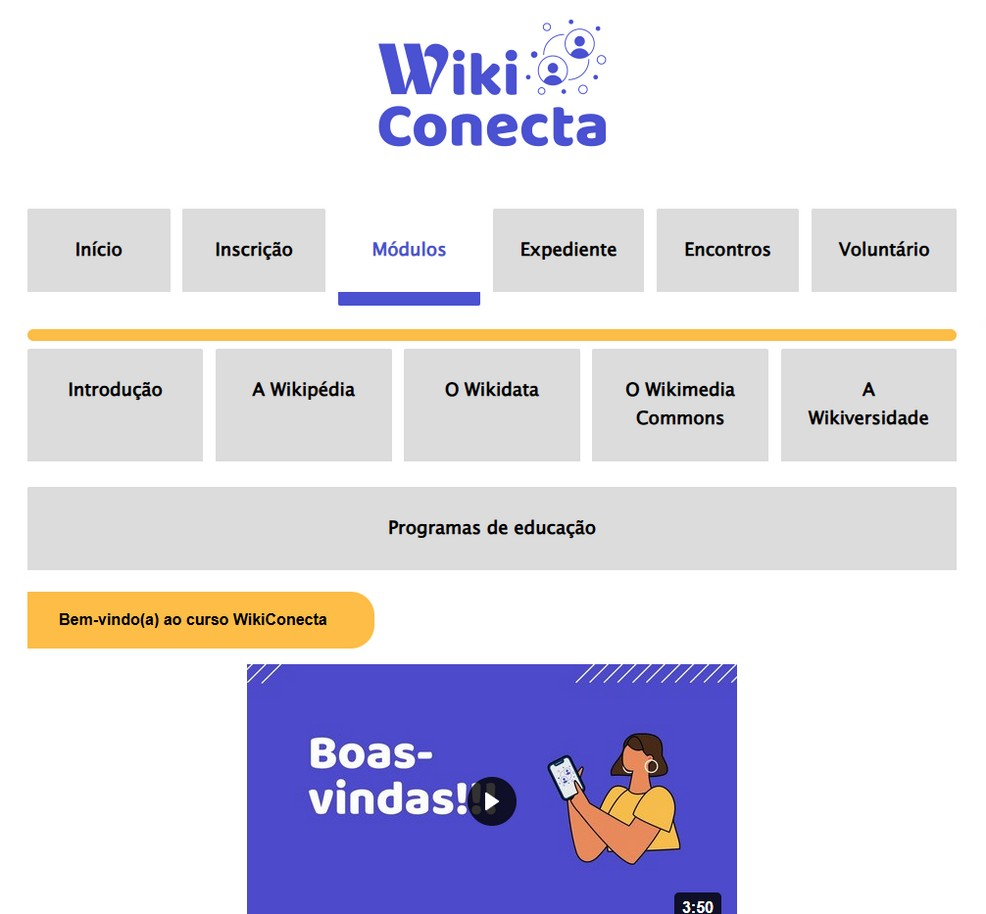
\includegraphics[width=\textwidth]{figures/figure03.jpg}
\caption{Vistas ortogonais e ortográficas: vista frontal; vista superior; e vista lateral esquerda.}
\label{fig-03}
\source{\url{http://turmag1215vialonga.blogspot.com/2014/10/projecoes-ortogonais.html}.}
\end{minipage}
\end{figure}

Posteriormente a professora apresentou a aplicabilidade das POs, dizendo
que eram destinadas à planificação de vários objetos. Com o auxílio das
simulações computacionais, construiu os sólidos geométricos e demonstrou
suas vistas ortogonais, apresentando os procedimentos para a manipulação
do Q3DM. (Ver \Cref{fig-04})

\begin{figure}[htpb]
\centering
\begin{minipage}{.5\textwidth}
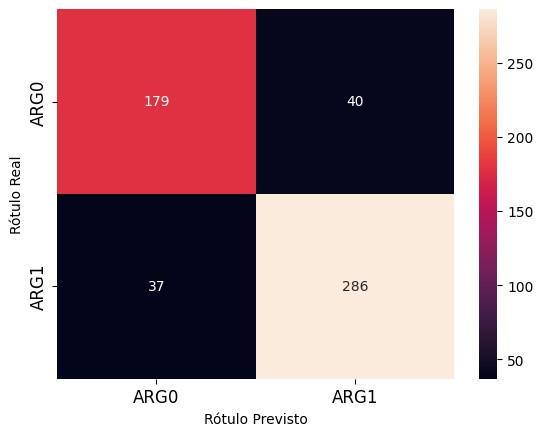
\includegraphics[width=\textwidth]{figures/figure04.jpg}
\caption{Manipulação no Q3DM.}
\label{fig-04}
\source{Elaboração própria.}	
\end{minipage}
\end{figure}


A manipulação no Q3DM é feita por meio de cubos chamados Qubes, que
facilitam a criação e a montagem de objetos em três dimensões,
utilizando elementos digitais que podem ser inseridos, removidos,
deslocados, ampliados, inclinados, moldados geometricamente, girados e
coloridos.

Para os alunos da 12ª classe, o tema de pesquisa foi SCs e foi utilizado
o GeoGebra. A professora iniciou com a apresentação do tema SCs de
cilindro, explicando que a seção cilíndrica é uma figura resultante de
um plano secante no cilindro. A professora acrescentou que existem duas
situações distintas: quando o plano secante é paralelo ao eixo central
do cilindro; e quando o plano secante não é paralelo ao eixo central do
cilindro (ver as figuras \Cref{fig-05} e \Cref{fig-06}).

\begin{figure}[htpb]
\centering
\begin{minipage}{.25\textwidth}
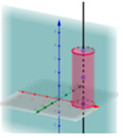
\includegraphics[width=\textwidth]{figures/figure05.jpg}
\caption{Secção paralela ao eixo central do cilindro.}
\label{fig-05}
\source{Elaboração própria.}
\end{minipage}
\end{figure}

\begin{figure}[htpb]
\centering
\begin{minipage}{.5\textwidth}
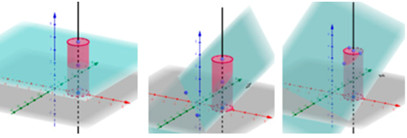
\includegraphics[width=\textwidth]{figures/figure06.jpg}
\caption{Secção não paralela ao eixo central do cilindro.}
\label{fig-06}
\source{Elaboração própria.}
\end{minipage}
\end{figure}

A professora, primeiramente, apresentou os diferentes posicionamentos
dos planos em relação ao eixo central do cilindro. Em seguida, com o
auxílio da tecnologia, apresentou à turma o software de geometria
dinâmica GeoGebra, indicando as funcionalidades de suas ferramentas e
como construir do ponto até o plano secante, com a ajuda dos
procedimentos para a sua manipulação no GeoGebra. Os alunos simularam as
SCs com o plano de nível; eles apresentaram-se atentos e motivados em
aprender a resolver o exercício no GeoGebra, particularmente para os
rapazes, os quais procuravam descobrir como construir diferentes sólidos
geométricos e como simular as VOs (vistas ortogonais).

\subsection{Realização do questionário}\label{sub-sec-Realização do questionário}

O questionário de satisfação aplicado teve como objetivo compreender se
o Q3DM e o GeoGebra facilitaram a aprendizagem das POs e SCs, e se o
\textit{smartphone} foi fácil de manipular. Ambos os questionários foram
preenchidos em 10 minutos. As questões visavam a coletar, nos dois
estudos, várias opiniões, incluindo: (1) se os aplicativos tecnológicos
facilitaram as representações 3D; (2) qual é a opinião deles sobre os
benefícios de usar os aplicativos ou se seria melhor resolver de forma
tradicional; (3) se os aplicativos são fáceis e intuitivos de usar; (4)
quais foram os aspectos positivos e negativos da aula; e, (5) como eles
classificariam a aprendizagem com o auxílio dos aplicativos.

\section{Análise}\label{sec-análise}

Nesta seção, realizaremos a análise dos 21 artigos selecionados para a
revisão sistemática de literatura sobre o conceito de literacia
algorítmica (LA). Todos os artigos analisados estão detalhados em tabela
no (\Cref{anexo-1}), que inclui o nome dos/das autores/as, ano da
publicação, título do artigo, tipo e local de publicação. Inicialmente,
apresentaremos uma análise dos metadados das publicações, entre eles o
ano de publicação, autores, periódicos ou eventos em que foram
apresentadas, junto a outros detalhes relevantes. Em seguida, realizamos
efetivamente a análise do \emph{corpus}, considerando as questões que
dirigem nossa investigação.

\subsection{Perspectivas iniciais a partir dos metadados}\label{sub-sec-perspectivasiniciais}

Ao analisar a lista de publicações, observamos que os dados abrangem um
período de quatro anos, de 2019 a 2022 (\Cref{image-02}). Notadamente, a
maioria das publicações se concentra nos anos de 2021 e 2022, quando
encontramos, respectivamente, 6 e 10 publicações. Essa concentração do
debate sobre o conceito de LA nos últimos quatro anos, assim como a
tendência ascendente do número de publicações sobre o tema, pode indicar
o aumento do reconhecimento da importância da compreensão dos algoritmos
e seus papéis na vida social contemporânea, bem como o avanço das
discussões em torno da LA.

\begin{figure}[!h]
\centering
\begin{minipage}{0.85\linewidth}
\caption{Número de publicações por ano.}
\label{image-02}
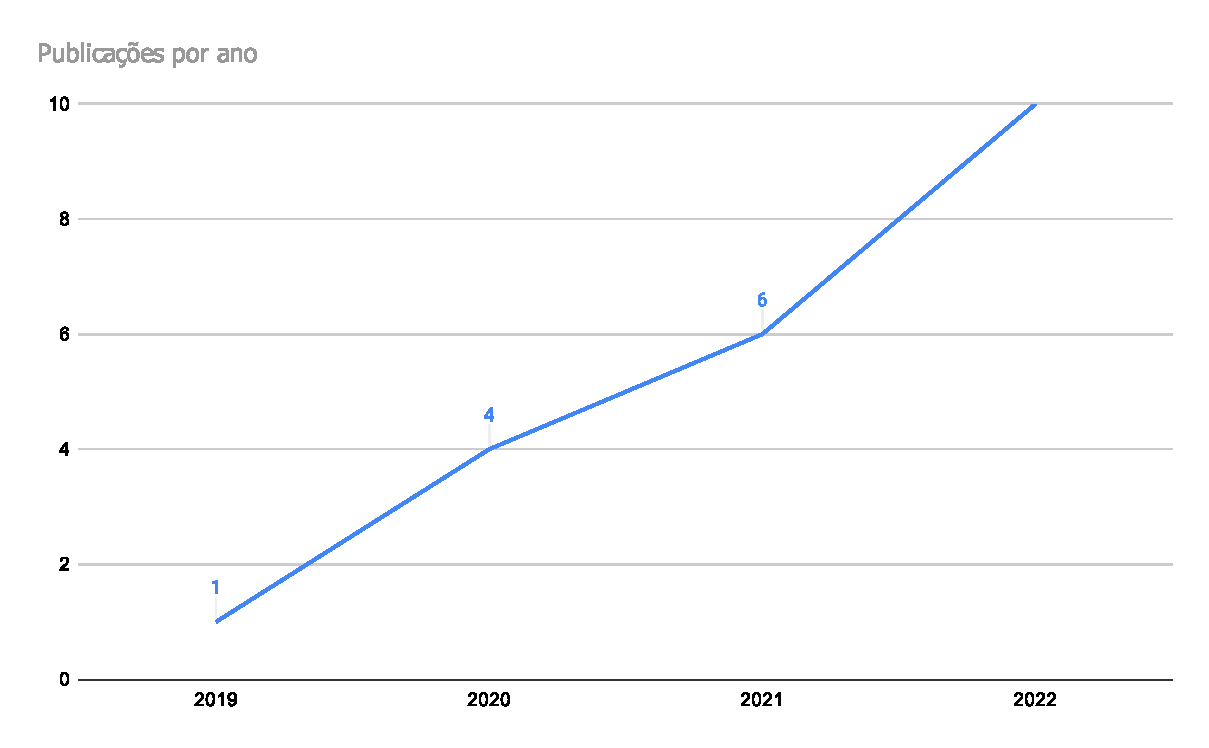
\includegraphics[width=\linewidth]{image2.pdf}
\source{Elaboração própria.}
\end{minipage}
\end{figure}

Em relação à origem das publicações, é possível observar uma diversidade
de formatos, abrangendo artigos em periódicos (15), capítulos de livros
(2) e artigos em anais de eventos acadêmicos (4). Conforme se vê na
tabela do \Cref{anexo-1}, apenas dois periódicos contêm mais de um artigo sobre
o tema (\emph{AI and Society} e \emph{Computers and Composition}).
Nota-se que os estudos encontrados abarcam uma ampla gama de áreas:
comunicação, computação, psicologia, ciência da informação, educação,
além de outras disciplinas relacionadas ao debate sobre tecnologias da
informação e comunicação (como a Interação Humano-Computador). Esse
aspecto pode indicar o interesse multidisciplinar no tema e a relevância
da noção de LA em diversos contextos acadêmicos.

Nessa etapa da análise, também foi percebida a ausência de textos em
português e o baixo número de publicações em espanhol entre os 21
artigos selecionados para a revisão sistemática sobre LA. Essa
observação pode indicar um cenário de escassez de investigações sobre o
tema no contexto latino e ibero-americano.

Com essas informações como base, a próxima etapa da nossa análise
aprofunda o estudo dessas publicações, considerando as questões
orientadoras da investigação sobre propostas conceituais, técnicas
pedagógicas, aplicações práticas e dificuldades relacionadas à LA.

\subsection{Explorando os fundamentos da literacia algorítmica: modelos
conceituais, distinções e aplicações multidisciplinares}\label{sub-sec-explorandoosfundamentos}

A análise dos artigos que abordam a LA revela um cenário diversificado e
complexo, no qual não se observa uma unidade conceitual. Inicialmente,
nota-se que o debate em torno da LA tem propostas que derivam de
abordagens de literacia preexistentes e mais consolidadas, como a
literacia informacional, a literacia para o ambiente digital e a
literacia para os dados \cite{Lloyd2019}. Essas abordagens enfatizam o
processo de criação de consciência individual sobre como a informação é
produzida, classificada e distribuída em diferentes ambientes \cite{Bakke2020}. Nestes estudos, a LA emerge como resposta aos efeitos da
introdução da agência algorítmica, uma série de competências mais
específicas no cenário de uma vida dataficada \cite{Kampa2021}.
Neste contexto, os apelos por literacias são frequentemente uma resposta
a novas tecnologias que criam novas estruturas de poder \cite{Devito2021}.

Para \textcite[p.~3]{Ridley2021}, LA é um dos desdobramentos das
variadas literacias do mundo digitalizado: ``Embora cada uma delas tenha
seu próprio domínio e foco, elas compartilham ideias comuns e geralmente
são simbióticas entre si'' \textcite[p.~3]{Ridley2021}. De modo
similar, \textcite[p.~30]{Devito2021} sustenta que a LA não deve ser observada
isoladamente, mas sim como ``um componente de uma literacia de
plataforma mais ampla que abrange todas as literacias mencionadas
anteriormente''. Para \cite{Lloyd2019}, o que difere a LA de propostas de
literacias mais gerais é que ela necessita de um exame aprofundado da
cultura de desenvolvimento desses sistemas, movimento que vai ao
encontro de propostas de investigação como a de \textcite{Seaver2017}. ``De
acordo com esta perspectiva, a construção de um algoritmo é uma prática
que está inserida dentro de outras práticas e é influenciada por visões
específicas do mundo'' \cite[p.~1483]{Lloyd2019}.

Nesse contexto, a especificidade da LA em relação a outras abordagens
pedagógicas do digital reside na necessidade de um exame crítico de
propriedades características da agência algorítmica, a partir de noções
como performatividade, opacidade, diversidade, confiança, viés e justiça
social \cite{Lloyd2019}. Complementarmente, \textcite{Devito2021} indica que
qualquer proposta de LA deve lidar com a natureza movediça dos sistemas
algorítmicos em constante transformação, incorporando nas construções
pedagógicas essa flexibilidade e capacidade de atualização. Para a
autora, isso faz com que seja fundamental reconhecer que ``os sujeitos
já estão imersos no ambiente em questão, tornando a LA um exercício
principalmente de formalizar e corrigir o conhecimento encontrado no
mundo, em vez de introduzir conhecimentos puramente novos'' \cite[p.~3–4]{Devito2021}.

Nos estudos analisados, um dos objetivos centrais para a LA é o
desenvolvimento de consciência sobre a agência dos sistemas algorítmicos
nas diferentes interações com os sujeitos \cite{Bakke2020}, seja na busca
por informações e conteúdos \cite{Kampa2021}, na interação com
sistemas de interação automatizados \cite{Shin2022} ou na relação com a
personalização algorítmica \cite{Devito2021,Lv2022,Bell2023}. Trata-se, segundo \textcite{Ridley2021},
de uma maneira de reconhecer e dar consciência sobre as formas de poder
deste padrão tecnológico e, ao mesmo tempo, enfatizar os empoderamentos
possíveis aos sujeitos diante dessas estruturas. Nesta abordagem, a LA
pode ser definida como a capacidade de estar ciente tanto da presença
quanto dos desdobramentos de sistemas conduzidos algoritmicamente e,
assim, cristalizar essa compreensão em um uso estratégico desses
sistemas para que os sujeitos integrantes desse processo possam alcançar
objetivos individuais ou coletivos \cite{Devito2021}. Dessarte, LA deve ser
entendida como mais do que instruções para um uso mais eficiente de
sistemas algorítmicos. Ela é uma prática ideológica de produção de
sentido e de subjetivações dissonantes ao que a performatividade desses
sistemas permite \cite{Ridley2021}.

No próximo segmento deste item da análise, serão exploradas duas
dimensões constituintes dos debates que emergem dos artigos examinados.
Primeiramente, será discutido o significado da noção de empoderamento
crítico. Depois, será abordado o espectro dos diferentes níveis de
consciência dos sujeitos em relação aos sistemas algorítmicos. Ambos os
debates são centrais para as propostas conceituais de LA analisadas.

\subsection{Empoderamento crítico: caminhos da agência diante de
sistemas algorítmicos}\label{sub-sec-empoderamentocritico}

Poder e controle são duas noções centrais no debate estabelecido pela
literatura crítica sobre algoritmos. \textcite{Magalhaes2018} sustenta que parte
da literatura, que chama de \emph{paradigma do dano}, considera o poder
dos algoritmos como resultado e também como impulsionador de uma
disparidade original entre os sujeitos (que têm suas vidas afetadas pela
análise de dados digitais sem estarem cientes disso) e os operadores das
plataformas (que deliberada e estrategicamente controlam a coleta e a
análise desses dados). Conforme indica \textcite{Rieder2018}, essas abordagens
estão orientadas, muitas vezes, a apenas denunciar os efeitos políticos
e sociais dos sistemas algorítmicos, negligenciando a análise de como
essas infraestruturas se articulam material e discursivamente para
produzir os efeitos de poder.

Na análise dos artigos da amostra, nos parece claro que poder e controle
são questões para as quais as investigações analisadas buscam oferecer
algum tipo de resposta ou abordagem crítica. Neles, a LA tende a ser
posicionada enquanto conhecimento pedagógico para o desenvolvimento de
consciência crítica e, consequentemente, ampliação da capacidade de
agência dos sujeitos. É neste contexto que emerge a noção de
\emph{empoderamento crítico} como resultado esperado da LA. Nas
propostas conceituais analisadas há ênfase em um empoderamento
individual a partir da capacidade de observar criticamente os modos de
funcionamento desses sistemas \cite{Bakke2020,Konig2022}.

\textcite{Konig2022}, por exemplo, sustenta que a LA pode formar sujeitos com
uma postura reflexiva em relação a sistemas algorítmicos, permitindo que
compreendam que, a cada sugestão ou resultado gerado por esses sistemas,
há trações de objetivos, interesses e suposições que não necessariamente
estão claros. De modo similar, \textcite[p.~1483]{Lloyd2019} entende que os
processos de reflexão são centrais nas literacias, por isso podem
colaborar para gerar atenção sobre como ``os algoritmos são expressos e
operacionalizados (por meio de nossas ações e interações com interfaces
e programas), juntamente com as condições, suposições e vieses que são
inerentes à sua produção e operacionalização.'' \textcite[p.~177]{Sued2022}
indica que a consciência crítica e o conhecimento desenvolvidos a partir
da LA podem garantir aos sujeitos ``um maior agenciamento e liberdade de
ação''.

Porém, adverte \textcite{Konig2022}, o \emph{empoderamento crítico} como
resultado da LA revela-se limitado por duas razões. Primeiramente, o
efeito de uma compreensão crítica dos algoritmos é naturalmente
restrito, já que não há garantias de que as pessoas poderão incorporar
esses conhecimentos e atitudes para exercer controle sobre as operações
de um sistema algorítmico. As configurações, interfaces e regras desses
sistemas, muitas vezes, atuam para limitar as possibilidades de escolha
individual. Mesmo que seja possível conceder aos usuários mais controle
por meio de influência individual sobre a configuração e o comportamento
do sistema, permanece um segundo obstáculo: a produção de uma postura
mais ativa e engajada desses sujeitos no processo de definição dos seus
objetivos, interesses e valores dentro desses sistemas.

Portanto, no debate sobre LA, a capacidade de desenvolver uma
consciência crítica em relação a sistemas algoritmos é vista como
caminho para ampliar a agência dos sujeitos, uma resposta crítica. Nesse
sentido, em conformidade com a abordagem de \textcite{Siles2024}, consideramos
que o debate sobre LA está imbricado com a noção de agência. Ao olhar o
que as pessoas fazem com os algoritmos, \textcite{Siles2024} propõe uma
abordagem de agência mais fluida, que deriva da bricolagem entre
discussões dos Estudos Culturais e dos Estudos de Ciência e Tecnologia.
Nessa proposta, a relação com algoritmos passa a ser vista menos como
polos opostos sólidos ou estados definitivos e mais como relações de
convergência, instabilidade, coexistência, fricção e mudança. Às vezes
os usuários seguem as sugestões dos algoritmos, outras vezes resistem a
elas. Muitas vezes, têm as duas posturas nas mesmas ações. Passa-se a
considerar que a agência é um processo relacional que se dá no espaço
intermediário da relação entre sujeitos e algoritmos \cite{Siles2024}.

No próximo item, são discutidas reflexões sobre os diferentes níveis de
consciência sobre o funcionamento de sistemas algorítmicos, um ponto de
destaque na literatura acerca do tema.

\subsection{Níveis de consciência e percepção sobre algoritmos}\label{sub-sec-niveisdeconscienciaepercepção}

A consciência sobre a existência e funcionamento de algoritmos é um tema
recorrente nas discussões sobre plataformas digitais. As pesquisas
iniciais, realizadas na metade da década anterior, indicaram um baixo
nível de consciência sobre a existência e o funcionamento dos algoritmos
\cite{Eslami2015}. \textcite{Bucher2019}, por exemplo, investigou o
modo como as pessoas tomam consciência sobre a agência algorítmica,
sugerindo que os imaginários sobre o funcionamento desses sistemas podem
condicionar a forma como esses indivíduos desenvolvem suas práticas em
uma determinada plataforma.

Nos debates observados em nosso estudo, a percepção dos sujeitos sobre
algoritmos é posicionada como fator central na literacia algorítmica
(LA), a partir da premissa de que as formas de compreensão sobre esses
sistemas podem moldar significativamente as práticas e interações dos
sujeitos com os ambientes digitais. Nos estudos observados na amostra
analisada, notam-se diferentes abordagens que dialogam com esta questão.
\textcite{Bell2023} apontam que a consciência sobre o
funcionamento de sistemas algorítmicos pode variar dramaticamente em um
grupo semelhante. No estudo, indica-se que a percepção sobre sistemas
algorítmicos pode variar entre plataformas e costuma ser mais
verbalizada quando se fala de serviços nos quais sistemas de
personalização são mais proeminentes no uso, como o TikTok \cite{Bell2023}. Segundo as autoras, essa percepção inclusive pode
depender da maneira como o tema é colocado aos sujeitos (por exemplo, a
partir da variação dos termos escolhidos, como algoritmo ou
personalização). Já a pesquisa de \textcite{Lv2022} correlaciona
essa consciência com a intenção dos adolescentes de resistir aos
algoritmos em plataformas \textit{on-line}. Para as autoras, os diferentes níveis
de conscientização e conhecimento sobre algoritmos estão relacionados à
disposição de os adolescentes buscarem formas de lidar ou evitar esses
sistemas \cite{Lv2022}. O estudo de \cite[p.~352]{Parnell2022}, que analisa as consultas a buscadores \textit{on-line}, apresenta
achados empíricos que indicam que ``uma maior literacia algorítmica tem
um efeito positivo nas habilidades autorrelatadas no uso de sistemas de
busca e no uso mais frequente da Internet''.

É possível perceber nesses estudos um esforço para a criação de
parâmetros que tornem possível mensurar graus de consciência e
conhecimento sobre sistemas algorítmicos. Seriam graus de LA que podem
ser identificados a partir das práticas dos sujeitos. Uma das propostas
que mais avança nesse propósito é a de \textcite{Devito2021}. A autora busca
estabelecer categorias para estratificar esses diferentes níveis de
consciência e conhecimento, que nomeia como Níveis de Complexidade da
Teorização do Indivíduo. Os graus de entendimento observados pela autora
são desenvolvidos, principalmente, a partir das \emph{folk theories}, ou
teorizações informais, como resultado da experiência dos sujeitos em
suas relações com sistemas algorítmicos e, ao mesmo tempo, do contato
com outros conteúdos que abordam o tema. Tais conteúdos passam a ser
incorporados nos modos como esses sujeitos organizam suas práticas
\cite{Devito2021}.

A estratificação proposta pela autora está dividida em dois níveis que
têm, cada um, subdivisões: a primeira é o dos Teóricos Funcionais, que
retrata os sujeitos que têm consciência inicial e compreensão limitada
dos aspectos funcionais dos algoritmos. Essa categoria é dividida em
\emph{Consciência Básica} (quando o sujeito identifica que um sistema
algorítmico está em operação em uma plataforma, tendo algum efeito, mas
não afirma ou consegue refletir sobre qual efeito específico) e
\emph{Poderes Causais} (quando o sujeito indica que um sistema
algorítmico é causa de um dado resultado). O segundo nível é o dos
Teóricos Estruturais, que destaca os sujeitos que fazem ajustes
substanciais em suas táticas para lidar diretamente com as questões
algorítmicas, expandindo suas fontes de informação. Essa categoria é
dividida por \textcite{Devito2021} em \emph{Fragmentos Mecanicistas} (quando o
sujeito indica que um sistema algorítmico desempenha papéis específicos
em uma plataforma e acredita que identificou múltiplos fatores que são
ponderados pelo sistema para tomar decisões) e \emph{Ordenamento
Mecanicista} (quando o sujeito percebe que um sistema algorítmico
desempenha papéis específicos em uma plataforma e acredita que
identificou não apenas múltiplos fatores usados para tomar decisões, mas
também a ordem de aplicação desses critérios ou o peso relativo de cada
um deles).

Portanto, a percepção e o conhecimento dos sujeitos sobre algoritmos
emergem como questões cruciais no contexto da LA. A literatura analisada
demonstra que a compreensão desses sistemas pode variar
significativamente entre os sujeitos e as plataformas observadas,
variação que pode influenciar consideravelmente suas interações e
práticas digitais. Além disso, pesquisas empíricas sugerem que níveis
mais elevados de consciência sobre algoritmos estão relacionados a uma
maior disposição para criar modos mais estratégicos de interação com
esses sistemas. A categorização proposta por \textcite{Devito2021} para
estratificar os diferentes níveis de consciência e conhecimento sobre
algoritmos oferece uma abordagem interessante para avaliar e compreender
essas diferenças. Porém, é necessário destacar o papel contingente que
os usos e práticas individuais podem ter no âmbito da relação com
algoritmos, assim como a já citada natureza movediça desses sistemas.
Esses fatores tornam limitadas qualquer proposta generalizante sobre
níveis de percepção e conhecimento.

\subsection{As propostas pedagógicas no contexto da literacia
algorítmica}\label{sub-sec-aspropostaspedagogicas}

A análise desenvolvida em nosso estudo possibilitou observar nos artigos
estudados um conjunto de propostas pedagógicas desenvolvidas com o
objetivo de promover o conhecimento e a consciência acerca da atuação de
sistemas algorítmicos. É interessante notar que as propostas observadas
não formam um conjunto uniforme metodologicamente. Há diferentes
percursos para o desenvolvimento da LA, apresentados a seguir.

Ao tentarem sistematizar os caminhos metodológicos da LA, \textcite{Silva2022} indicam duas possíveis vias. A primeira consiste na
construção de conhecimentos básicos a partir da exploração dos objetivos
dos desenvolvedores desses sistemas e dos efeitos dessas tecnologias em
nossas sociedades. Essa abordagem, que classificamos como conteudista, é
desenvolvida através da oferta de informações sólidas sobre os
propósitos subjacentes aos algoritmos e como eles afetam diferentes
dimensões da vida cotidiana. A segunda via concentra-se na produção de
experiência a partir da interação com sistemas algorítmicos. Nesse caso,
os aprendizes são incentivados a explorar as funcionalidades dos
algoritmos, buscando desenvolver seus esquemas e conhecimentos para
explicar como eles funcionam e como suas decisões são tomadas.

Explorar as experiências desenvolvidas pelos sujeitos em contato com
sistemas algorítmicos também é uma proposta pedagógica central do estudo
de \textcite{Devito2021}. Como já destacado, a autora centra sua discussão no
âmbito das \emph{folk theories} para ``explicar os resultados, efeitos
ou consequências de sistemas tecnológicos'' \cite[p. 4]{Devito2021}. Essa
proposta tem como premissa a noção de que já temos, em maior ou menor
medida, alguma experiência com esses sistemas, portanto a LA deve ser
principalmente o exercício de formalizar e corrigir o conhecimento
encontrado no mundo, em vez de puramente introduzir novos conhecimentos
\cite{Devito2021}. O propósito metodológico da LA defendida por \textcite{Devito2021} é desenvolver modos de aprendizagem que levem os sujeitos a um
entendimento estrutural desses sistemas. Isso implica tanto em
compreender que os algoritmos têm um efeito em resultados específicos
quanto em identificar os diversos fatores específicos que são ponderados
pelos algoritmos e a ordem em que esses critérios são aplicados.

Já \textcite{Ridley2021} ancoram-se na literatura sobre
pensamento computacional para o desenvolvimento de propostas pedagógicas
no campo da LA. Para os autores, essas duas noções guardam uma
interessante correlação e, por isso, a extensa literatura sobre
pensamento computacional é considerada por eles como frutífera para a LA
\cite{Ridley2021}. Os autores consideram que tal aproximação
pode ajudar a desenvolver uma compreensão sobre algoritmos e seus
processos, interpretar seus usos em diferentes sistemas, além de criar e
aplicar técnicas e ferramentas algorítmicas para resolver problemas em
uma variedade de domínios.

No caminho do desenvolvimento pedagógico a partir das experiências,
\textcite{Klumbbyte2020} discutem a promoção da LA por meio de
abordagens pedagógicas que utilizam o design crítico para a interação
com algoritmos. A proposta dos autores centra-se na ideia do
desenvolvimento do \textit{Social Privilege Estimator}, um sistema de pontuação
social baseado em reconhecimento facial e classificação, que foi
construído como um artefato de design crítico para conscientizar sobre
as desigualdades existentes e os efeitos adversos dos sistemas de
reconhecimento facial. Também no campo do design, \textcite{Cech2020} propõe um
debate sobre medidas de co-design como suporte ao desenvolvimento de LA
e da compreensão dos processos algorítmicos. Por meio de princípios de
design participativo e centrado no usuário, a autora sugere o desenho
colaborativo de soluções materiais e processuais para a compreensão dos
processos algorítmicos e de promoção nesses sistemas.

Por fim, observamos propostas que estabelecem o que nomeamos de
interação narrativa como método para o desenvolvimento da LA:
metodologias pedagógicas que estão baseadas no desenvolvimento de
experiências a partir de propostas narrativas, como jogos e dinâmicas,
nos quais os sujeitos são convidados a atuar e tomar decisões como se
fossem desenvolvedores desses sistemas. \textcite[p.~199]{Aleman2021} apresentam a proposta de um jogo digital no qual os sujeitos são
colocados em interação com ``uma narrativa envolvente e um ambiente de
programação que demonstram as limitações dos modelos preditivos''. A
proposta dos autores busca levar educadores e estudantes a examinarem os
vieses de modelos algorítmicos e, assim, fomentar a reflexão sobre as
tensões com sistemas algorítmicos em suas vidas.

De modo similar, \textcite{Jeong2022} propõem a implementação de
iniciativas educativas com foco no sistema de recomendação do YouTube a
partir de uma dinâmica que busca colocar estudantes do ensino
fundamental na pele do algoritmo, como responsáveis pelas definições do
que é relevante na plataforma. A proposta dos autores é inspirada pela
metodologia desenvolvida por \textcite{Grosman2022}, que
consiste em uma dinâmica que oferece aos participantes dados e objetivos
para a realização de sugestões musicais no YouTube. Conforme \textcite{Jeong2022}, a proposta tem como objetivo incentivar os jovens a
compreenderem como algoritmos de recomendação funcionam e afetam as
interações dos sujeitos com o YouTube.

Ainda no contexto da sala de aula, \textcite{Koenig2020} propõe a produção
textual em diários como metodologia pedagógica de incentivo às reflexões
de estudantes sobre suas interações com as plataformas. A proposta do
autor consiste basicamente na criação de diários individuais para
explorar e refletir sobre suas próprias interações com sistemas
algorítmicos. Incentiva a reflexão sobre as experiências dos alunos com
plataformas a partir da produção textual sobre experiências e hábitos. A
partir do experimento empírico conduzido, \textcite{Koenig2020} indica que os
alunos se tornaram mais críticos e conscientes sobre o funcionamento de
plataformas.

A análise das propostas pedagógicas indica que há diferentes caminhos
metodológicos que buscam promover o conhecimento e a consciência acerca
da atuação de sistemas algorítmicos. As propostas observadas podem
variar de abordagens mais tradicionais, conteudistas, nas quais
almeja-se informar os sujeitos sobre a ação de algoritmos, até
abordagens mais relacionais, nas quais os sujeitos são convidados a
experienciar novos modos de interação com esses sistemas.

\section{Considerações finais}\label{sec-consideraçõesfinais}

Nosso estudo teve como objetivo mapear o campo de investigação sobre
literacia algorítmica (LA) nas línguas portuguesa, espanhola e inglesa.
Para isso, foram utilizados quatro eixos: a definição de propostas
conceituais, a identificação de técnicas e estratégias pedagógicas
emergentes, a descrição das funções e domínios dessas diferentes formas
de conhecimento e a reflexão sobre os desafios e dificuldades revelados
na literatura.

A respeito das propostas conceituais (Q1), observamos um conjunto
diversificado de abordagens, que, embora faça referências a literacias
preexistentes, possui especificidades que o diferenciam. De modo geral,
o que difere a LA de propostas predecessoras de literacia é o foco
crítico na agência dos sistemas algorítmicos, considerando sua natureza
performática e mutável.

Quanto às abordagens pedagógicas (Q2), apesar do número restrito de
publicações sobre o tema, é percebida uma diversidade de estratégias em
torno do ensino e da conscientização sobre algoritmos. Dentre essas
abordagens, destacam-se as metodologias conteudistas, que buscam
informar os sujeitos dos desdobramentos da relação com algoritmos, e as
metodologias experienciais, que incentivam a exploração das vivências e
conhecimentos desenvolvidos nas interações com sistemas algorítmicos.
Propostas de design crítico, interação em jogos, produção textual e
dinâmicas narrativas também emergem como metodologias que almejam
envolver os sujeitos no processo de compreensão e crítica. Sobre as
áreas de conhecimento nas quais se localizam os debates sobre LA (Q3),
consideramos ser possível afirmar que se trata de um objeto de pesquisa
eminentemente transdisciplinar. Em nosso estudo, percebe-se uma
significativa amplitude de campos de conhecimentos nas quais o tema vem
sendo estudado, como comunicação, computação, educação, psicologia e
ciência da informação. Quanto às dificuldades percebidas nos estudos
analisados (Q4), consideramos que o desafio central para o campo de
investigação está na falta de uma definição clara e consistente do
conceito, junto à sua proximidade com outras formas de literacia. No que
tange ao desenvolvimento de consciência crítica, os estudos analisados
referem dificuldades relacionadas à própria natureza frequentemente
opaca e complexa dos sistemas algorítmicos, sobretudo para compreensão e
agência sobre seu funcionamento e desdobramentos. Também são referidas
como dificuldades as desigualdades no acesso a tecnologias digitais.

Em conclusão, a LA é uma área emergente e transdisciplinar que carece de
desenvolvimento tanto conceitual, para maior clareza, quanto
metodológico, com o desenvolvimento de propostas que possam auxiliar no
processo de promoção de consciência e senso crítico diante das ações dos
algoritmos. Podemos posicioná-la como uma série de conhecimentos e
dinâmicas que almejam produzir consciência sobre a agência dos
algoritmos nas relações e que se estabelecem nas ambiências das
plataformas. As diferentes abordagens da LA costumam emprazar modos
pelos quais os sujeitos possam utilizar estrategicamente esses sistemas
para alcançar objetivos pessoais e coletivos. Diferente de outras formas
de literacia, a LA exige um exame crítico das práticas de
desenvolvimento dos sistemas algorítmicos, abordando questões como
performatividade, opacidade, viés e justiça social.


\section*{Financiamento} O presente trabalho foi realizado com apoio da
Coordenação de Aperfeiçoamento de Pessoal de Nível Superior - Brasil (CAPES) -
Código de Financiamento 001. O estudo foi realizado também com o apoio do
projeto `Percepción y generación de conocimiento sobre los algoritmos de
personalización en las plataformas digitales de comunicación - ALCOM' código
PID2023-148682OA-I00, financiado pelo Ministério de Ciência, Inovação e
Universidades da Espanha.

\printbibliography\label{sec-bib}
%conceptualization,datacuration,formalanalysis,funding,investigation,methodology,projadm,resources,software,supervision,validation,visualization,writing,review
\begin{contributors}[sec-contributors]
\authorcontribution{Willian Fernandes Araujo}[conceptualization,methodology,writing,review]
\authorcontribution{Fernanda Pires de Sá}[methodology,writing]
\end{contributors}

\appendix
\section*{Anexo}\label{anexo-1}

\setlength\LTleft{-0.8in}
\setlength\LTright{-0.8in}
\begin{footnotesize}
\begin{longtable}{
    >{\raggedright\arraybackslash}p{0.2\textwidth}
    >{\raggedright\arraybackslash}p{0.075\textwidth}
    >{\raggedright\arraybackslash}p{0.4\textwidth}
    >{\raggedright\arraybackslash}p{0.125\textwidth}
    >{\raggedright\arraybackslash}p{0.2\textwidth}
    }
\caption{Local de publicação de acordo com área de concentração e natureza} \label{tab-anexo-1}\\
\\
\toprule
Autores(as) & Ano & Título do texto &Tipo &Fonte da publicação\\
\midrule
Lloyd, A. & 2019 & Chasing Frankenstein's monster: information literacy
in the black box society & Artigo em Periódico & Journal of
Documentation \\
Bakke, A. & 2020 & Everyday Googling: Results of an Observational Study
and Applications for Teaching Algorithmic Literacy & Artigo em Periódico
& Computers and Composition \\
Cech, F. & 2020 & Beyond transparency: Exploring algorithmic
accountability & Texto publicado em anais de eventos & Proceedings of
the International ACM SIGGROUP Conference on Supporting Group Work \\
Klumbyte, G.; Lücking, P.; Draude, C. & 2020 & Reframing AX with
Critical Design: The Potentials and Limits of Algorithmic Experience as
a Critical Design Concept & Texto publicado em anais de eventos & 11th
Nordic Conference on Human-Computer Interaction: Shaping Experiences,
Shaping Society (NordiCHI '20), \\
Koenig, A. & 2020 & The Algorithms Know Me and I Know Them: Using
Student Journals to Uncover Algorithmic Literacy Awareness & Artigo em
Periódico & Computers and Composition \\
Aleman, E.; Nadolny, L.; Ferreira, A.; Gabetti, B.; Ortíz, G.;
Zanoniani, M. & 2021 & Screening bot: A playground for critical
algorithmic literacy engagement with youth & Texto publicado em anais de
eventos & CHI PLAY 2021 - Extended Abstracts of the 2021 Annual
Symposium on Computer-Human Interaction in Play \\
DeVito, M.A. & 2021 & Adaptive Folk Theorization as a Path to
Algorithmic Literacy on Changing Platforms & Artigo em Periódico &
Proceedings of the ACM on Human-Computer Interaction \\
Kampa, P.; Balzer, F. & 2021 & Algorithmic literacy in medical students
-- results of a knowledge test conducted in Germany & Artigo em
Periódico & Health Information and Libraries Journal \\
Reisdorf, B.C.; Blank, G. & 2021 & Algorithmic literacy and platform
trust & Capítulo de livro & Handbook of Digital Inequality \\
Ridley, M.; Pawlick-Potts, D. & 2021 & Algorithmic literacy and the role
for libraries & Artigo em Periódico & Information Technology and
Libraries \\
Swart, J. & 2021 & Experiencing Algorithms: How Young People Understand,
Feel About, and Engage With Algorithmic News Selection on Social Media &
Artigo em Periódico & Social Media and Society \\
Bell, A.R., Tennfjord, M.K., Tokovska, M., Eg, R. & 2022 & Exploring the
role of social media literacy in adolescents\textquotesingle{}
experiences with personalization: A Norwegian qualitative study & Artigo
em Periódico & Journal of Adolescent and Adult Literacy \\
Dogruel, L., Masur, P., Joeckel, S. & 2022 & Development and Validation
of an Algorithm Literacy Scale for Internet Users & Artigo em Periódico
& Communication Methods and Measures \\
Jeong, H.-S., Oh, Y.J., Kim, A. & 2022 & CRITICAL ALGORITHM LITERACY
EDUCATION IN THE AGE OF DIGITAL PLATFORMS: Teaching children to
understand YouTube recommendation algorithms & Capítulo de livro &
Learning to Live with Datafication: Educational Case Studies and
Initiatives from Across the World \\
König, P.D. & 2022 & Challenges in enabling user control over
algorithm-based services & Artigo em Periódico & AI and Society \\
Lv, X., Chen, Y., Guo, W. & 2022 & Adolescents' Algorithmic Resistance
to Short Video APP's Recommendation: The Dual Mediating Role of
Resistance Willingness and Resistance Intention & Artigo em Periódico &
Frontiers in Psychology \\
Parnell, S.I., Klein, S.H., Gaiser, F. & 2022 & Do we know and do we
care\textquotesingle{} Algorithms and Attitude towards Conversational
User Interfaces: Comparing Chatbots and Voice Assistants & Texto
publicado em anais de eventos & 4th Conference on Conversational User
Interfaces (CUI 2022) \\
Shin, D. & 2022 & How do people judge the credibility of algorithmic
sources? & Artigo em Periódico & AI and Society \\
Shin, D., Rasul, A., Fotiadis, A. & 2022 & Why am I seeing this?
Deconstructing algorithm literacy through the lens of users & Artigo em
Periódico & Internet Research \\
Silva, D.E., Chen, C., Zhu, Y. & 2022 & Facets of algorithmic literacy:
Information, experience, and individual factors predict attitudes toward
algorithmic systems & Artigo em Periódico & New Media and Society \\
Sued, G.E. & 2022 & TRAINING THE ALGORITHM: GOVERNANCE, AGENCY, AND
LITERACY IN THE USE OF YOUTUBE {[}Entrenar al algoritmo: gobernanza,
agencia y literacidad en el uso de YouTube{]} & Artigo em Periódico &
Contratexto \\
\bottomrule
\source{Elaboração própria.}
\end{longtable}
\end{footnotesize}


\end{document}
